\subsection{Desarrollo de la idea.}

\vspace*{0.3cm}

Sea $G$ un grafo cualquiera, $I$ un conjunto independiente de ese nodo, y $n_{1}$,$n_{2}$ nodos de G que no pertenecen a $I$ y no tienen aristas en común con ningún elemento de $I$, diremos que $n_{1}$ es óptimo si no existe ningún $n_{2}$ tal que $( \# (Vecinos(n_{2})) - \# (Vecinos(n_{2}) \cap Vecinos(I))) > ( \# (Vecinos(n_{1})) - \# (Vecinos(n_{1}) \cap Vecinos(I)))$. Definimos $Vecinos(\alpha)$ como el conjunto de nodos a los cuales $\alpha$ lleva una arista si $\alpha$ es un nodo, y si $\alpha$ es un conjunto, entonces es el conjunto de nodos a los cuales les llega un arista desde por lo menos un elemento de $\alpha$.  De manera más informal, podemos decir que un nodo óptimo es aquél que más vecinos ``libres'' tiene, siendo un nodo ``libre'' uno que no está en el conjunto solución ni es adyacente a un nodo de la solución.

Nuestra heurística se basa en formar un conjunto independiente maximal de la siguiente manera:
Primero, considerando al conjunto independiente vacío, tomamos a un nodo óptimo, y lo agregamos como nuevo elemento de nuestro conjunto independiente. Luego con nuestro nuevo conjunto independiente, tomamos un nodo óptimo, y lo agregamos a nuestro conjunto independiente. Repetimos esto hasta que no exista un nodo óptimo, puesto que nuestro conjunto independiente se transformó en maximal, y por lo tanto en un conjunto dominante.
 
\vspace*{0.6cm}

%\newpage

\subsection{Análisis de complejidad.}

\vspace*{0.3cm}

Pasemos a analizar la complejidad del algoritmo en cuestión, tal vez abstrayendonos del peor caso, pero si tratando de maximizar los costos de los distintos pasos a realizar. Notemos primero que buscar el nodo ``óptimo'' nos toma $\mathcal{O}(n)$ ya que se trata de recorrer los nodos del grafo haciendo comparaciones sobre la cantidad de vecinos que possen $\mathcal{O}(1)$. (Creo que no sería errado decir que si entro $n$ veces a buscar al optimo, es porque todos tenian grado 0, sino se irian eliminando posibilidades, por ende la complejidad seria $\mathcal{O}(n^2)$).


Supongamos un caso en el que debo entrar $n-1$ veces a buscar el ``óptimo'' $\mathcal{O}(n)$. Luego tendría un costo de $\mathcal{O}(n^2)$.


A este se le suma el costo de marcar a los nodos elegidos y a sus vecinos como ``tomados''. Para esto debemos tener en cuenta que marcarlos toma $\mathcal{O}(1)$, y que cada nodo puede tener como máximo $n-1$ vecinos, pero la suma total de nodos vecinos a marcar como tomados es siempre $n-1$ ($\mathcal{O}(n)$). Luego, y ya metiéndonos un poco con lo que respecta a la implementación, debemos actualizar los grados de los nodos vecinos de los vecinos del nodo tomado como ``óptimo''. Como ya dijimos, la suma de los vecinos del nodo tomado puede llegar a $n-1$, y estos a su vez podrían llegar a tener $n-1$ vecinos. Como debo recorrerlos para actualizarlos estaríamos hablando de una complejidad de $\mathcal{O}(n^2)$


Por último la solución del algoritmo consiste integrar cada nodo ``óptimo'' a la solución final, lo que puede llegar a tomar $\mathcal{O}(n)$.

Siendo $T(n)$ la complejidad de nuestro algoritmo tenemos:

\begin{equation*}
\begin{array}{l}
T(n) = \mathcal{O}(n^2) + \mathcal{O}(n) + \mathcal{O}(n^2)\\
T(n) = 2\mathcal{O}(n^2)
T(n) = \mathcal{O}(n^2)
\end{array}
\end{equation*}

\begin{figure}
\begin{codebox}
\Procname{$\proc{CIDM_goloso}(lista\_nodos$ $cidm\_sol)$} 
\li $res \leftarrow$ 0
\li \While no se hayan ``tomado'' todos los nodos
\li 	\Do 
 		$elegido \leftarrow$ nodo ``óptimo''
\li 		$cidm\_sol \leftarrow$ agregar $elegido$
\li 		incrementar $res$
\li 		marcar a $elegido$ y a sus vecinos como ``tomados''
	\End
\li \Return $res$
\end{codebox}
\caption{Heurística golosa constructiva para CIDM}\label{code:goloso}
\end{figure}
%\FloatBarrier

\vspace*{0.6cm}
%\newpage

\subsection{Instancias no óptimas.}

\vspace*{0.3cm}

A continuación presentaremos dos familias de grafos para las cuales nuestra heurística golosa no siempre encuentra una solución óptima.

\subsubsection*{Familia 1 - Estrellas}

La forma de los grafos pertenecientes a esta familia responde a las siguientes características:

\begin{itemize}
\item Existe un único vértice $v$ con grado máximo.  Sea $\delta_{max}$ el grado de este nodo.
\item Para cada vértice $w$ adyacente a $v$, $\delta(w) < \delta_{max}$, y sus nodos adyacentes (salvo $v$) tienen grado 1.	
\end{itemize}

Dado que el algoritmo propuesto va tomando en cada paso el nodo ``óptimo'', o sea, aquél que más nodos ``libres'' cubre, en un grafo como el descrito primero tomará al vértice $v$ con grado máximo $\delta_{max}$.  Luego, para cumplir con la independencia y la dominancia, deberá tomar a los vértices adyacentes a los vecinos de $v$. Como el grado de cada vecino de $v$ es menor a $\delta_{max}$, el peor de los casos sería que cada uno de ellos tuviera grado $\delta_{max} - 1$.  En este caso, cada vértice adyacente a $v$ tendría $\delta_{max} - 2$ vecinos además del mismo $v$, y entonces la solución hallada por nuestra heurística estaría conformada por $\delta_{max} \times (\delta_{max} - 2)$ nodos.  Sin embargo, para un grafo como el detallado, existe una solución mejor conformada por $\delta_{max}$ nodos, y corresponde al conjunto compuesto por los vecinos del nodo $v$.

La Figura \ref{fig:familia1} muestra un ejemplo de grafo perteneciente a esta familia, y la Figura \ref{fig:familia1res} muestra en color verde la solución hallada por nuestro algoritmo, la cual claramente es peor que la solución formada por los vértices que quedaron en rojo en la misma Figura.

\begin{figure}[!htb]
\minipage{0.5\textwidth}
\begin{center}
  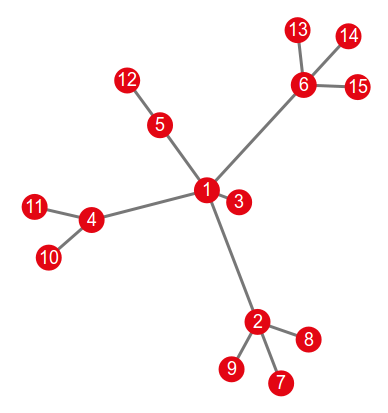
\includegraphics[scale=0.5]{imagenes/familia1.png}
\end{center}
  \caption{Grafo perteneciente a la Familia 1}\label{fig:familia1}
\endminipage\hfill
\minipage{0.5\textwidth}
\begin{center}
  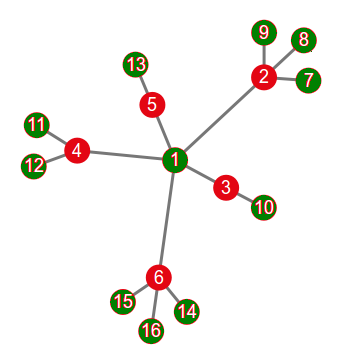
\includegraphics[scale=0.5]{imagenes/familia1-res.png}
\end{center}
  \caption{Solución hallada por nuestra heurística}\label{fig:familia1res}
\endminipage
\end{figure}

\subsubsection*{Familia 2 - Circuitos}

Como miembros de esta familia consideraremos a los circuitos simples.  Para este tipo de grafos, la calidad de la solución hallada por nuestro algoritmo dependerá de la cantidad de vértices que tenga y de la forma en que se hayan rotulado los mismos.

Consideremos un circuito $C_{n}$ y supongamos por un momento que los vértices están rotulados como $v_0,v_1,...,v_{n-1}$ tal que existe una arista entre $v_i$ y $v_j$ cuando $j = (i+1) mod (n)$.

1. Una forma de armar un conjunto independiente maximal $C$ para este grafo podría ser la siguiente:

\begin{itemize}
\item Si $n \equiv 0 (3)$, tomar $C = \{v_i | i \equiv 1 (3)\}$.
\item Si $n \equiv 1 (3)$, tomar $C = \{v_i | i \equiv 1 (3)\} \cup \{v_{n-1}\}$.
\item Si $n \equiv 2 (3)$, tomar $C = \{v_i | i \equiv 1 (3)\}$.
\end{itemize}

2. Veamos que $C$ efectivamente es independiente maximal, y por lo tanto, dominante.

\paragraph*{Independencia:} Cuando $n \equiv 0 (3)$, el conjunto $C$ está formado por los vértices $v_i$ tal que $i \equiv 1 (3)$, por lo cual $v_i$ se comunica con $v_{i-1}$ y con $v_{i+1}$. Como $i-1 \equiv 0 (3)$ y $i+1 \equiv 2 (3)$, entonces los vértices incluidos en $C$ no se comunican entre sí. Cuando $n \equiv 1 (3)$ ó $n \equiv 2 (3)$, todo lo antes escrito también vale, considerando que $v_{n-1}$ (que en ambos casos pertenece a $C$) tiene por vecinos a $v_{n-2}$ y $v_{0}$, y sucede que $0 \equiv 0 (3)$ y $n-2 \equiv 2 (3)$ ó $n-2 \equiv 0 (3)$, por lo cual sigue cumpliéndose la independencia.

\paragraph*{Maximalidad:} Supongamos que $C$ no es maximal, es decir, que podemos incluir al menos un vértice más y seguir teniendo un conjunto independiente. Analicemos los siguientes casos:

\begin{itemize}
	\item Agregar un vértice $v_i$ tal que $i \equiv 1 (3)$.  Pero todos ya forman parte de $C$. ABSURDO.
	\item Agregar un vértice $v_i$ tal que $i \equiv 2 (3)$.  Pero todos se encuentran conectados al vértice $v_{i-1}$ y como en este caso $i-1 \equiv 1(3)$, entonces por definición $v_{i-1} \in C$. ABSURDO.
	\item Agregar un vértice $v_i$ tal que $i \equiv 0 (3)$.  Pero entonces $v_i$ o bien se conecta al vértice $v_{i+1}$ con $i+1 \equiv 1 (3)$ y por lo tanto $v_{i+1} \in C$, o bien $i = n-1$ cuando $n \equiv 1 (3)$ así que también pertenece a $C$. ABSURDO.
\end{itemize}

Luego, $C$ es un conjunto independiente maximal, y por consiguiente, dominante. 

3. Veamos ahora que $C$ también es mínimo (o sea, un CIDM de $C_n$).

Primero, diremos que, dentro de un grafo, un vértice $v$ ``cubre'' a un vértice $w$ o bien cuando $v = w$, o bien cuando $v$ y $w$ son adyacentes. Por lo tanto, un vértice $v$ cubre exactamente a $\delta(v) + 1$ vértices.

Particularmente, dado un CIDM para un determinado grafo $G = (V,E)$, entre todos los vértices pertenecientes a dicho conjunto ``cubren'' a todos los vértices de $G$ (porque es dominante). Notemos además, que dos vértices diferentes del CIDM pueden cubrir a un mismo vértice dentro de $G$ (es decir, pueden tener vecinos en común). Entonces, si tomamos un CIDM $S$ para $G$, y sabiendo que cada vértice $v \in S$ cubre a $\delta(v) + 1$ vértices dentro de $G$, podemos decir que 

\begin{equation*}
\sum_{v \in S} \text{nodos cubiertos por }v = |S| + \sum_{v \in S} \delta(v) \geq |V|
\end{equation*}

Volviendo ahora a nuestro conjunto independiente maximal $C$ del circuito $C_n$ definido anteriormente. En principio, fácilmente vemos su cardinalidad:

\begin{itemize}
	\item Cuando $n \equiv 0 (3), |C| = \frac{n}{3}$.
	\item Cuando $n \equiv 1 (3), |C| = \frac{n-1}{3} + 1$.	
	\item Cuando $n \equiv 2 (3), |C| = \frac{n-2}{3} + 1$.	
\end{itemize}

Para probar que $C$ es un CIDM, supongamos que no lo es.  Es decir, que existe un conjunto independiente y dominante $C'$ con menor cardinalidad que $C$.  Podemos decir que $|C'| = |C| - k$ para algún $k \in [1, |C|)$. Como $C_n$ es un circuito simple, cada vértice tiene grado exactamente 2.  Entonces,

\begin{equation*}
\sum_{v \in C'} \text{nodos cubiertos por }v = |C'| + \sum_{v \in C'} \delta(v) = |C'| + 2|C'| = 3 |C'| = 3(|C| - k) = 3|C| - 3k
\end{equation*}

\begin{itemize}
	\item Cuando $n \equiv 0 (3), 3|C| - 3k = 3\frac{n}{3} - 3k = n-3k < n$ pues $k$ es al menos 1. ABSURDO.
	\item Cuando $n \equiv 1 (3), 3|C| - 3k = 3(\frac{n-1}{3} + 1) - 3k = n+2-3k < n$ pues $k$ es al menos 1. ABSURDO.
	\item Cuando $n \equiv 2 (3), 3|C| - 3k = 3(\frac{n-2}{3} + 1) - 3k = n+1-3k < n$ pues $k$ es al menos 1. ABSURDO.
\end{itemize}

Luego, concluimos que $C$ es un CIDM de $C_n$.

4. Supongamos ahora que vamos armando al conjunto $C$ tomando los nodos $v_i$ de la manera indicada anteriormente, pero de forma secuencial, de menor a mayor valor de $i$. Notamos entonces que:

\begin{itemize}
	\item Cuando $n \equiv 0 (3)$, cada vértice $v_i$ que se incluye en $C$ cubre exactamente 3 vértices ``libres'' (sus dos vecinos y él mismo).
	\item Cuando $n \equiv 1 (3)$, cada vértice $v_i$ que se incluye en $C$ tal que $i \equiv 1 (3)$ también cubre exactamente 3 vértices ``libres'', y por último $v_{n-1}$ sólo se cubre a sí mismo, ya que sus vecinos fueron cubiertos anteriormente por $v_1$ y $v_{n-3}$.
	\item Cuando $n \equiv 2 (3)$, cada vértice $v_i$ que se incluye en $C$ tal que $i \equiv 1 (3)$ también cubre exactamente 3 vértices ``libres'', y por último $v_{n-1}$ se cubre a sí mismo y a $v_{n-2}$, ya que $v_0$ fue cubierto anteriormente por $v_1$.
\end{itemize}

Por lo tanto, podemos decir que al momento de tomar cada vértice de $C$, el mismo califica como nodo ``óptimo''.

5. Definimos ahora la siguiente función $f:V \rightarrow \mathbb{N} \in (0,n]$ para rotular los vértices de $C_n$:

\begin{equation*}
f(v_i) = \begin{cases}
\dfrac{i-1}{3}+1 & \text{si } i \equiv 1 (3)\\\\
k \in (|C|,n] \text{ no utilizado aún} & \text{si no}
\end{cases}
\end{equation*}

6. Por una decisión implementativa, nuestra heurística golosa va tomando secuencialmente los nodos ``óptimos'' en el orden en el que fueron rotulados (o sea que siempre toma el nodo ``óptimo'' con rotulado menor). Entonces, si tomamos un circuito $C_n$ donde los vértices son $v_0,v_1,...,v_{n-1}$ tal que existe una arista entre $v_i$ y $v_j$ cuando $j = (i+1) mod (n)$, podemos formar un conjunto $C$ como se indica en el punto 1, y sabemos por los puntos 2 y 3 que se trata de un CIDM.  Si además, rotulamos los vértices como se indica en el punto 5, podemos ver que, por lo dicho en el punto 4, nuestro algoritmo encuentra una solución exacta, idéntica al conjunto $C$. La Figura \ref{fig:familia2} muestra un ejemplo de circuito rotulado de la manera indicada, y la Figura \ref{fig:familia2res} muestra la respuesta hallada por nuestro algoritmo.


A. Ahora, considerando el circuito $C_n$ inicial, tomemos el siguiente conjunto de vértices $C = \{v_i |(i \equiv 1 (4)) \vee (i \equiv 3 (4))\}$.  Básicamente, tomamos los nodos $v_i$ tal que $i$ es impar.

B. Veamos que $C$ es independiente maximal, y por lo tanto, dominante.

\paragraph*{Independencia:} El conjunto $C$ está formado por los vértices $v_i$ tal que $i \equiv 1 (4)$ ó $i \equiv 3 (4)$. Si $n$ es impar, sabemos que $v_i$ se comunica con $v_{(i-1)}$ y con $v_{(i+1)}$. Si $i \equiv 1 (4)$ entonces $i-1 \equiv 0 (4)$ y $i+1 \equiv 2 (4)$, y si $i \equiv 3 (4)$ entonces $i-1 \equiv 2 (4)$ y $i+1 \equiv 0 (4)$, así que los vértices incluidos en $C$ no se comunican entre sí. Si $n$ es impar, todo lo antes escrito también vale, considerando que $v_{n-1}$ (que pertenece a $C$) tiene por vecinos a $v_{n-2}$ y $v_{0}$, y sucede que $0 \equiv 0 (4)$ y $n-2 \equiv 2 (4)$ ó $n-2 \equiv 0 (4)$, por lo cual sigue cumpliéndose la independencia.

\paragraph*{Maximalidad:} Supongamos que $C$ no es maximal, es decir, que podemos incluir al menos un vértice más y seguir teniendo un conjunto independiente. Analicemos los siguientes casos:

\begin{itemize}
	\item Agregar un vértice $v_i$ tal que $i \equiv 1 (4)$.  Pero todos ya forman parte de $C$. ABSURDO.
	\item Agregar un vértice $v_i$ tal que $i \equiv 3 (4)$.  Pero todos ya forman parte de $C$. ABSURDO.
	\item Agregar un vértice $v_i$ tal que $i \equiv 0 (4)$.  Pero todos se encuentran conectados al vértice $v_{i+1}$ y como en este caso $i+1 \equiv 1(4)$, entonces por definición $v_{i+1} \in C$. ABSURDO.
	\item Agregar un vértice $v_i$ tal que $i \equiv 2 (4)$.  Pero todos se encuentran conectados al vértice $v_{i-1}$ y como en este caso $i-1 \equiv 1(4)$, entonces por definición $v_{i+1} \in C$. ABSURDO.
\end{itemize}

Luego, $C$ es un conjunto independiente maximal, y por consiguiente, dominante. 

C. Veamos ahora que el conjunto $C$ es un conjunto independiente máximo.  Para ello observemos la cardinalidad de $C$ (la cual es trivial dado que sólo tomamos a los vértices $v_i$ con $i$ impar):

\begin{itemize}
	\item Cuando $n$ es par,$|C| = \frac{n}{2}$.
	\item Cuando $n$ es impar, $|C| = \frac{n-1}{2}$.	
\end{itemize}

Para probar que $C$ es un conjunto independiente máximo, supongamos que no lo es.  Es decir, que existe un conjunto independiente maximal $C'$ con mayor cardinalidad que $C$.  Podemos decir que $|C'| = |C| + k$ para algún $k \in [1, (n -|C|))$. Pero dada la cardinalidad de $C$, tener un conjunto con más elementos implicaría que dicho conjunto contiene a más de la mitad de los vértices del grafo, y como se trata de un circuito simple y cada vértice tiene grado 2, obliga a que al menos dos vértices de $C'$ sean adyacentes.  Esto es absurdo puesto que supusimos $C'$ independiente.  Entonces, $C$ es un conjunto independiente máximo.

D. Supongamos ahora que vamos armando al conjunto $C$ tomando los nodos $v_i$ de la manera indicada anteriormente, pero de forma secuencial, de menor a mayor valor de $i$ con $i \equiv 1 (4)$, y luego de menor a mayor valor de $i$ con $i \equiv 3 (4)$. Notamos entonces que:

\begin{itemize}
	\item Cuando tomamos los $v_i$ tal que $i \equiv 1 (4)$, cada uno cubre exactamente 3 vértices ``libres'' (sus dos vecinos y él mismo).
	\item Cuando pasamos a tomar los $v_i$ tal que $i \equiv 3 (4)$ $n \equiv 1 (3)$, cada uno sólo cubre 1 vértice ``libre'' que es él mismo.  Esto sucede porque sus dos vecinos fueron cubiertos anteriormente por los $v_i$ con $i \equiv 1 (4)$.
\end{itemize}

Por lo tanto, podemos decir que al momento de tomar cada vértice de $C$, el mismo califica como nodo ``óptimo''.

E. Definimos ahora la siguiente función $f:V \rightarrow \mathbb{N} \in (0,n]$ para rotular los vértices de $C_n$:

\begin{equation*}
f(v_i) = \begin{cases}
\dfrac{i-1}{4}+1 & \text{si } i \equiv 1 (4)\\\\
\dfrac{i-3}{4}+\left\lfloor \dfrac{n}{4} \right\rfloor + 1 & \text{si } i \equiv 3 (4) \wedge (n \equiv 0 (4) \vee n \equiv 1 (4))\\\\
\dfrac{i-3}{4}+\left\lceil \dfrac{n}{4} \right\rceil + 1 & \text{si } i \equiv 3 (4) \wedge (n \equiv 2 (4) \vee n \equiv 3 (4))\\\\
k \in \left(\dfrac{n}{2},n\right] \text{ no utilizado aún} & \text{si } (i \equiv 0 (4) \vee i \equiv 2 (4)) \wedge (n \equiv 0 (4) \vee n \equiv 2 (4))\\\\
k \in \left(\dfrac{n-1}{2},n\right] \text{ no utilizado aún} & \text{si } (i \equiv 0 (4) \vee i \equiv 2 (4)) \wedge (n \equiv 1 (4) \vee n \equiv 3 (4))\\\\
\end{cases}
\end{equation*}

F. Como hemos decidido nuestra heurística golosa vaya tomando secuencialmente los nodos ``óptimos'' en el orden en el que fueron rotulados, entonces si tomamos un circuito $C_n$ donde los vértices son $v_0,v_1,...,v_{n-1}$ tal que existe una arista entre $v_i$ y $v_j$ cuando $j = (i+1) mod (n)$, podemos formar un conjunto $C$ como se indica en el punto A, y sabemos por los puntos B y C que se trata de un conjunto independiente máximo, y por consiguiente, dominante.  Si además, rotulamos los vértices como se indica en el punto E, podemos ver que, por lo dicho en el punto D, nuestro algoritmo encuentra una solución idéntica al conjunto $C$. 

Hay una excepción para el caso $n \equiv 2 (4)$. En estos casos, el vértice $n-1 \equiv 1 (4)$, pero el vértice $v_{n-1}$ no será tomado por nuestro algoritmo dado que se conecta al vértice $v_0$ que ya fue cubierto por $v_1$ y sólo podría cubrir a su otro vecino y a él mismo como nodos ``libres'', así que en su lugar se tomará al vértice $v_{i-2}$ que puede cubrir a 3 vértices ``libres'' (él mismo, $v_{n-1}$ y $v_{n-3}$, ya que $n-3 \equiv 3 (4)$ y aún no fue tomado). Por consiguiente, al comenzar a tomar a los $v_i$ tales que $i \equiv 3 (4)$, $v_{n-3}$ no será tomado en cuenta ya que no está ``libre''.  Luego, cuando $n \equiv 2 (4)$, la solución hallada por nuestra heurística toma a todos los $v_i$ tal que $i \equiv 1 (4)$ salvo $v_{n-1}$, luego toma a $v_{i-2}$, y finalmente toma a todos los $v_i$ tal que $i \equiv 3 (4)$ salvo $v_{n-3}$.  El tamaño del conjunto hallado, entonces, difiere sólo en una unidad respecto al conjunto planteado en el punto A.

La Figura \ref{fig:familia2bis} muestra un ejemplo de circuito rotulado de la manera indicada, y la Figura \ref{fig:familia2bisres} muestra la respuesta hallada por nuestro algoritmo.

\vspace*{0.3cm}

Para poder comparar las soluciones halladas por nuestra heurística para los rotulados propuestos, aproximaremos la cardinalidad del conjunto encontrado a $\frac{n}{3}$ para el primer caso y $\frac{n}{2}$ para el último, ya que a valores de $n$ muy grandes, la diferencia respecto a $\frac{n-1}{3}+1$ y a $\frac{n-2}{3}+1$ para el primero, y a $\frac{n-1}{2}$ en el segundo, es despreciable.  Entonces podemos decir que la mejor solución para un circuito simple $C_n$ contiene $\frac{n}{3}$ elementos mientras que la peor solución hallada para el mismo circuito contiene $\frac{n}{2}$ elementos.  En otras palabras, para un rotulado como el propuesto en E, el conjunto encontrado por nuestro algoritmo es un $50\%$ peor que el exacto.


\begin{figure}[!htb]
\minipage{0.5\textwidth}
\begin{center}
  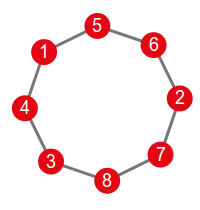
\includegraphics[scale=0.8]{imagenes/faimilia2.png}
\end{center}
  \caption{Circuito simple rotulado ``en orden''}\label{fig:familia2}
\endminipage\hfill
\minipage{0.5\textwidth}
\begin{center}
  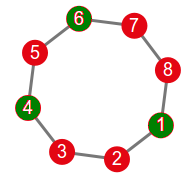
\includegraphics[scale=0.8]{imagenes/faimilia2-resopt.png}
\end{center}
  \caption{Solución hallada por nuestra heurística}\label{fig:familia2res}
\endminipage\\
\minipage{0.5\textwidth}
\begin{center}
  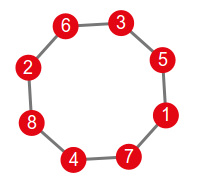
\includegraphics[scale=1.0]{imagenes/faimilia2rename.png}
\end{center}
  \caption{Circuito simple rotulado ``no en orden''}\label{fig:familia2bis}
\endminipage\hfill
\minipage{0.5\textwidth}
\begin{center}
  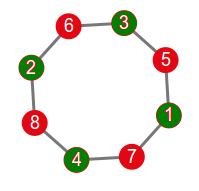
\includegraphics[scale=1.0]{imagenes/faimilia2rename-solnoopt.png}
\end{center}
  \caption{Solución hallada por nuestra heurística}\label{fig:familia2bisres}
\endminipage
\end{figure}



\vspace*{0.6cm}

\subsection{Instancias óptimas.}

\vspace*{0.3cm}

A continuación presentaremos una familia de grafos para la cual nuestra heurística golosa siempre encuentra una solución óptima.

La forma de los grafos pertenecientes a esta familia responde a las siguientes características:

\begin{itemize}
\item Existe un único vértice $v$ que llamaremos ``central'', con grado $\delta(v)$.
\item Para cada vértice $w$ adyacente a $v$, $\delta(w) > \delta(v)$, y sus nodos adyacentes (salvo $v$) tienen grado 1.	
\end{itemize}

Dado que el algoritmo propuesto va tomando en cada paso el nodo ``óptimo'', o sea, aquél que más nodos ``libres'' cubre, en un grafo como el descrito se irá formando el conjunto solución con los vértices adyacentes al nodo ``central'' $v$.  

FALTA MOSTRAR QUE ES LA MEJOR

La Figura \ref{fig:familia3} muestra un ejemplo de grafo perteneciente a esta familia, y la Figura \ref{fig:familia3res} muestra en color verde la solución hallada por nuestro algoritmo.

\begin{figure}[!htb]
\minipage{0.5\textwidth}
\begin{center}
  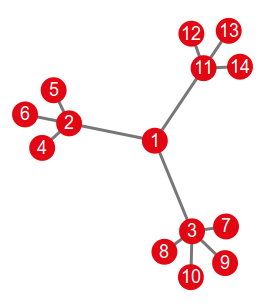
\includegraphics[scale=0.5]{imagenes/familia3.png}
\end{center}
  \caption{Grafo perteneciente a la Familia óptima}\label{fig:familia3}
\endminipage\hfill
\minipage{0.5\textwidth}
\begin{center}
  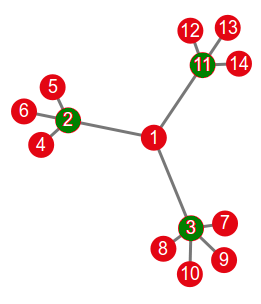
\includegraphics[scale=0.5]{imagenes/familia3-res.png}
\end{center}
  \caption{Solución hallada por nuestra heurística}\label{fig:familia3res}
\endminipage
\end{figure}


\vspace*{0.6cm}

\subsection{Experimentación y gráficos.}

\vspace*{0.3cm}

\vspace*{0.6cm}

\subsubsection{Test 1}
\vspace*{0.3cm}

\vspace*{0.6cm}
%\newpage

\subsubsection{Test 2}

